\begin{figure}
	\centering
	\begin{subfigure}{0.48\columnwidth}
		\centering
		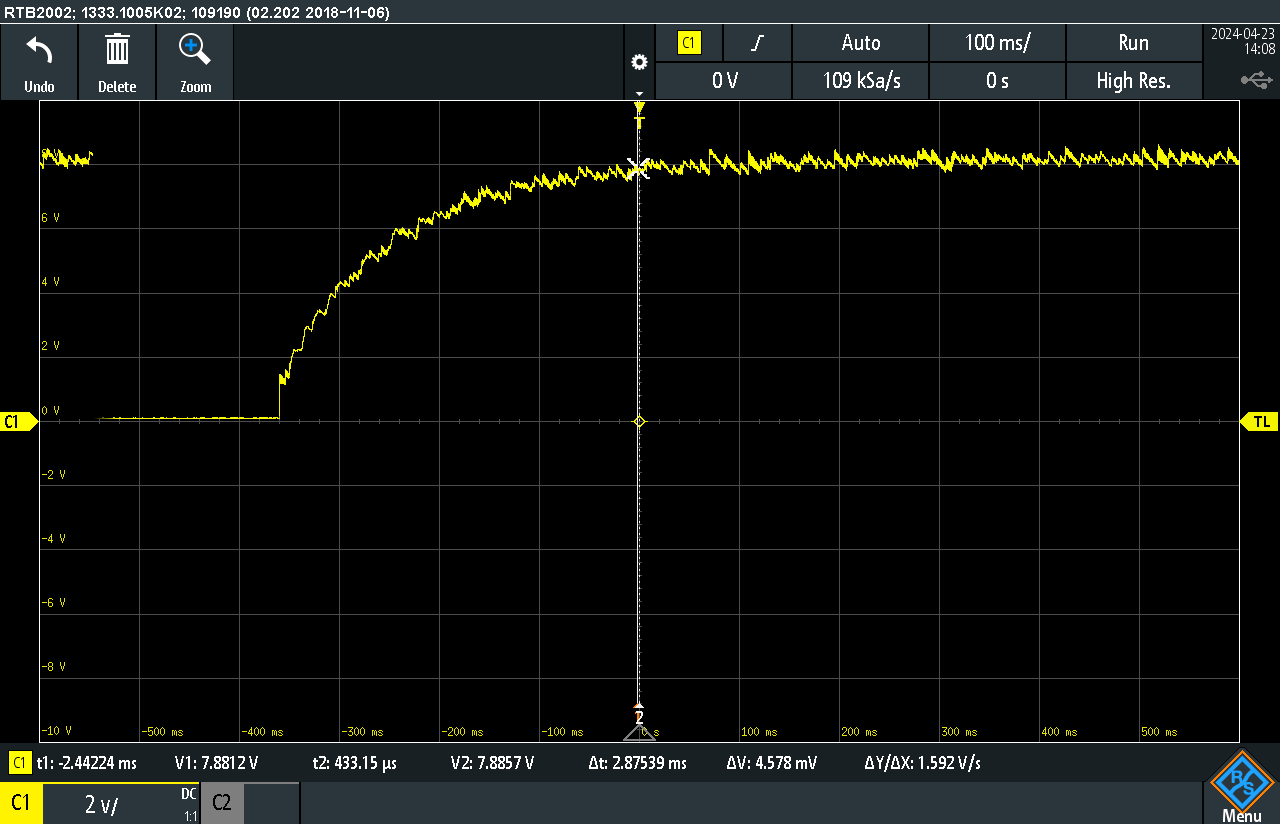
\includegraphics[width=0.8\linewidth]{src/figures/time-constant/1.PNG}
		\subcaption{1回目}
	\end{subfigure}
	\begin{subfigure}{0.48\columnwidth}
		\centering
		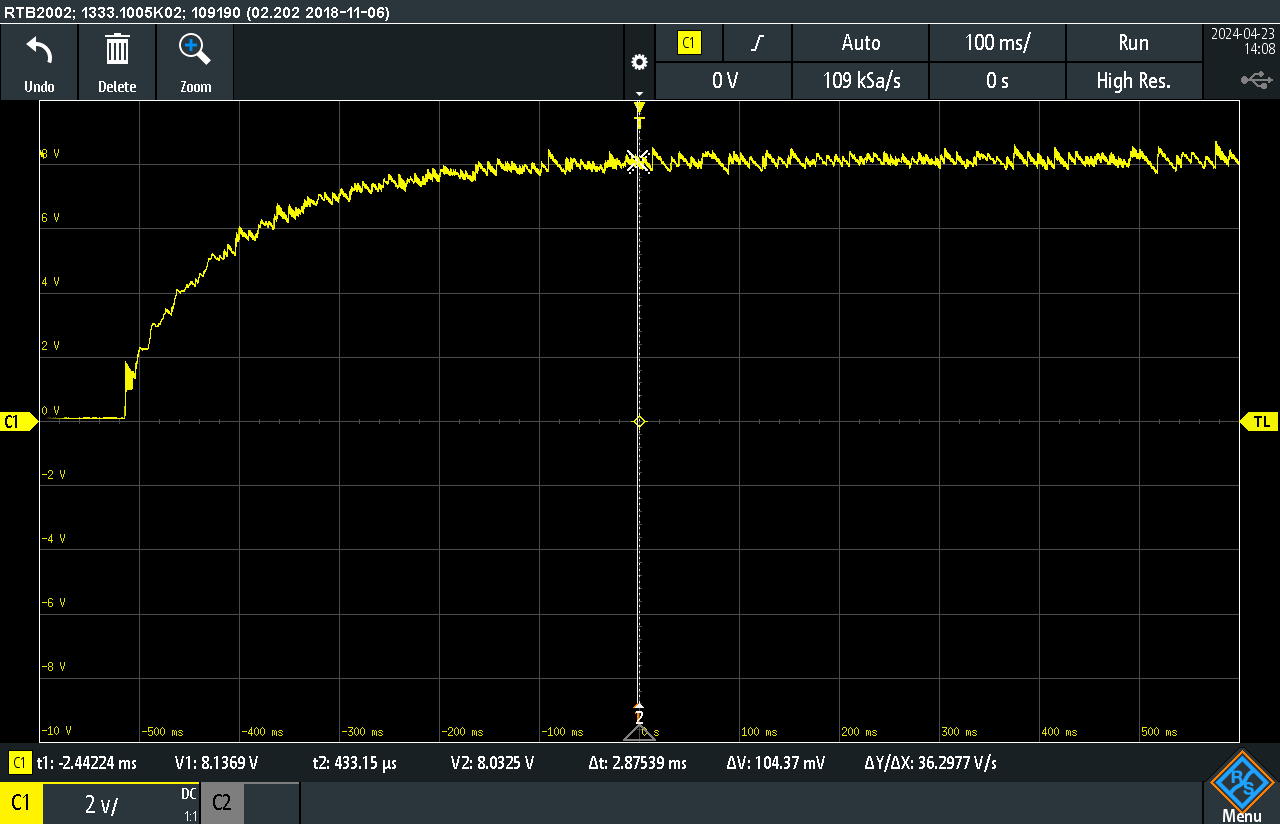
\includegraphics[width=0.8\linewidth]{src/figures/time-constant/2.PNG}
		\subcaption{2回目}
	\end{subfigure}
	\begin{subfigure}{0.48\columnwidth}
		\centering
		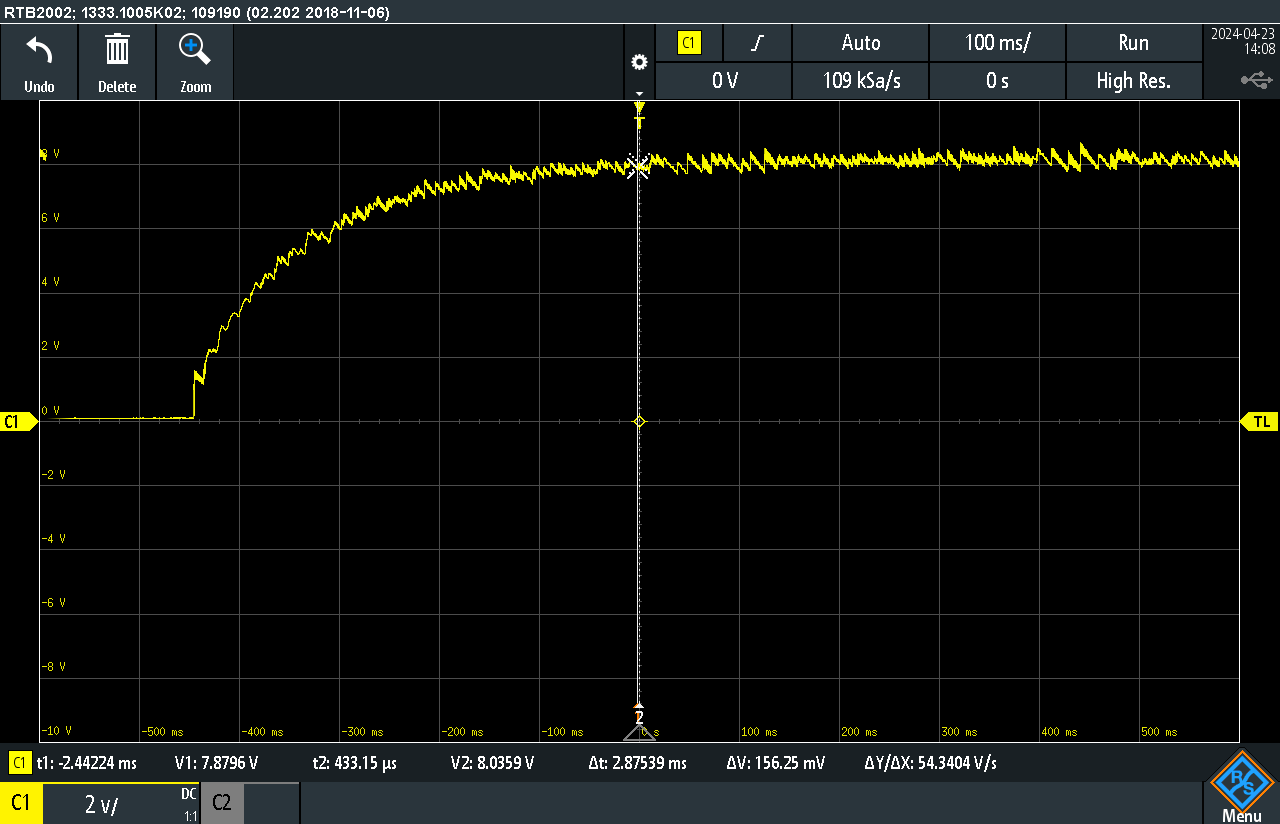
\includegraphics[width=0.8\linewidth]{src/figures/time-constant/3.PNG}
		\subcaption{3回目}
	\end{subfigure}
	\caption{時間定数の測定}\label{fig:time-constant}
\end{figure}
